\documentclass[12pt]{article}

\usepackage{graphicx}
\usepackage{indentfirst} % garante que a primeira linha terá identação.
\usepackage{listings}
\usepackage{xcolor}
\usepackage{hyperref}       % Permite o uso de hyperlinks no texto, com um link clicável
\usepackage{amsmath}

\definecolor{codegreen}{rgb}{0,0.6,0}
\definecolor{codegray}{rgb}{0.5,0.5,0.5}
\definecolor{codepurple}{rgb}{0.58,0,0.82}
\definecolor{backcolour}{rgb}{0.95,0.95,0.92}

\lstdefinestyle{mystyle}{
    backgroundcolor=\color{backcolour},   
    commentstyle=\color{codegreen},
    keywordstyle=\color{magenta},
    numberstyle=\tiny\color{codegray},
    stringstyle=\color{codepurple},
    basicstyle=\ttfamily\footnotesize,
    breakatwhitespace=false,         
    breaklines=true,                 
    captionpos=b,                    
    keepspaces=true,                 
    numbers=left,                    
    numbersep=5pt,                  
    showspaces=false,                
    showstringspaces=false,
    showtabs=false,                  
    tabsize=2
}

\lstset{style=mystyle}
\newcommand{\blue}[1]{\textcolor{blue}{#1}}

\title{S-DES, ECB e CBC}
\author{Gabriel Henrique do Nascimento Neres \\ Arthur Diehl Barroso}
\date{\today}

\begin{document}
\maketitle

\begin{abstract}
  Texto detalhando o desenvolvimento de uma versão simplificada do algoritmo de criptografia AES, denominado de S-AES, detalhando a implementação do modo de operação ECB. Além disso, é abordado as diferenças entre 5 modos de operação utilizando a biblioteca pyCryptoDome do python.

  \textbf{Palavras-chave}: Criptografia, AES, modos de operação.
\end{abstract}

Esse trabalho irá implementar e detalhar as etapas de confecção do algoritmo de criptografia simétrica S-AES, um modelo simplificado do algoritmo AES, com uso do modo de operação ECB. Em um segundo momento serão abordados 5 modos de operação que podem ser utilizados pelo algoritmo AES, sendo eles, \textbf{ECB}, \textbf{CBC}, \textbf{OFB}, \textbf{CFB} e \textbf{CTR}.

Para compreender melhor a implementação que está sendo feita, serão repassados os resultados de cada função desenvolvida baseado nos dados de entrada a baixo:

\begin{itemize}
  \item Chave: 1010011100111011
  \item Mensagem: 0110 1111 0110 1011 ("ok" em ASCII)
\end{itemize}

\section{S-AES}
O algoritmo de encriptação que estamos denominando de \textbf{S-AES} é uma forma simplificada do modelo AES que fará uso de uma chave de tamanho 16 bits, mensagens em blocos de 16 bits e a redução do número de rodadas para 2. A título de comparação, vale trazer que o \textbf{AES} possui blocos de 128 bits, chaves que podem ser de 128, 192 ou 256 bits e o número de rodadas para cada versão é, respectivamente, 10, 12 e 14 rodadas.

\textbf{OBS}: Neste trabalho a palavra "word" será utilizada para indicar um bloco de 1 byte (8 bits), o que difere da convenção de uma "word" indicar 4 bytes (32 bits). O termo foi mantido para permitir melhor correlação com a documentação do AES.

\subsection{Funções auxiliares}
\label{sec:funcoes_auxiliares}
As primeiras coisas que serão implementadas serão as funções responsáveis por fazer conversões entre um int de 16 bits e uma matriz 2x2 de nibbles, que denominaremos essa matriz de \textbf{estado}. 

Para essa conversão serão utilizados o operador "$>>$" com um \textbf{AND} com 0xF para conseguir quebrar o valor de 16 bits em 4 partes de 4 bits e o operador "$<<$" com uso do \textbf{OR} para reunir os 4 nibbles novamente em um inteiro de 16 bits.

A lógica utilizada na conversão para nibbles é manter, nessa ordem, os 4, 12, 8e 16 bits mais significativos e realizar um \textbf{AND} com 0xF para obter os 4 bits menos significativos do conjunto mantido, assim somos capazes de dividir o valor de 16 bits em 4 partes.

\begin{lstlisting}[language=Python]
def int_to_state(block: int) -> list[list[int]]:
  return [
    [(block >> 12) & 0xF, (block >> 4) & 0xF],
    [(block >> 8) & 0xF, block & 0xF]
  ]
\end{lstlisting}

Entrando com a chave de exemplo, teremos como saída a seguinte matriz:
$$
\begin{bmatrix}
10 & 3 \\
7 & 11 
\end{bmatrix}
$$

O processo inverso é feito seguindo a lógica de incluir zeros a direita de cada parte da matriz para obter um inteiro de 16 bits, unindo cada um dos 4 campos utilizando um \textbf{OR} após a inclusão dos zeros.

\begin{lstlisting}[language=Python]
def state_to_int(state: list[list[int]]) -> int:
  return (
    ((state[0][0] & 0xF) << 12) |
    ((state[1][0] & 0xF) << 8)  |
    ((state[0][1] & 0xF) << 4)  |
    (state[1][1] & 0xF)
  )
\end{lstlisting}

Em comparação com o algoritmo \textbf{AES}, a implementação do \blue{estado} segue uma estrutura diferente. No AES a matriz que foi denominada como estado possui tamanho 4x4 e cada parte possui comprimento de 8 bits.

\subsection{Expansão da chave e round-key}
Ao implementar o algoritmo, serão utilizadas 3 chaves ao longo do processo de encriptação. A primeira, utilizada antes da primeira rodada, será a própria chave passada ao algoritmo, já as outras duas serão derivadas utilizando uma função de expansão. 

Essa função irá seguir a lógica apresentada na imagem \ref{fig:Key Expansion} que poderá ser simplificada nas seguintes etapas:
\begin{itemize}
  \item Reunir as colunas da matriz em words;
  \item Executar a função g com a word 1;
  \item Realizar o XOR entre word 0 e o resultado da g;
  \item Realizar o XOR entre word 1 e a word 2 (gerada pelo XOR anterior);
\end{itemize}

\begin{figure}[h]
  \caption{Processo de expansão da chave}
    \centering
    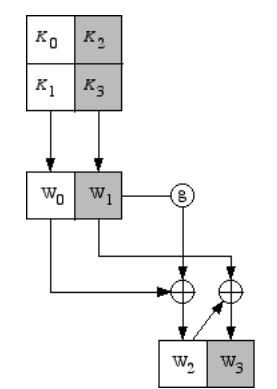
\includegraphics[width = 0.4\linewidth]{Imagens/Key-expansion.png}  
    \label{fig:Key Expansion}
\end{figure}

Esse processo resultará na chave utilizada pela primeira rodada do algoritmo, a outra cave será obtida utilizando a chave da primeira rodada na mesma função de expansão.

A função de expansão foi implementada da seguinte maneira:
\begin{lstlisting}[language=Python]
def expand_key(prev_key: list[list[int]], round_num: int) -> list[list[int]]:
  w0 = [prev_key[0][0], prev_key[1][0]]
  w1 = [prev_key[0][1], prev_key[1][1]]

  g_w1 = g(w1, round_num)

  w2 = [w0[0] ^ g_w1[0], w0[1] ^ g_w1[1]]
  w3 = [w2[0] ^ w1[0], w2[1] ^ w1[1]]

  return [[w2[0], w3[0]], [w2[1], w3[1]]]
\end{lstlisting}

Já a função g tem um conjunto de operações no seu interior, que são:
\begin{itemize}
  \item Divide a word nas suas duas metades;
  \item Inverte a posição das metades;
  \item Converte cada metade utilizado o conjunto de S-box do S-AES;
  \item Realiza o XOR entre cada metade pela constante de round, definida por $x^{j+2}$.
\end{itemize}

Assim, o código utilizado ficou como:
\begin{lstlisting}[language=Python]
def g(byte: list[int], round_num: int) -> list[int]:
  rcon = RCON[round_num]

  tmp_byte = sub_word(rot_word(byte))

  return [
    tmp_byte[0] ^ rcon[0],
    tmp_byte[1] ^ rcon[1]
  ]
\end{lstlisting}

Para exemplificar o processo de expansão da chave, utilizando a chave definida para esse trabalho teremos os resultados para as chaves 1, 2 e 3, além das etapas intermediárias do processamento apresentadas na imagem \ref{fig:Key Expansion Results} com valores em decimal e hexadecimal (prefixada com 0x). 

\begin{figure}[h]
    \centering
    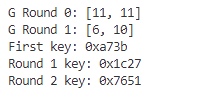
\includegraphics[width = 0.35\linewidth]{Imagens/Key-expansion-results.png}  
    \label{fig:Key Expansion Results}
\end{figure}

No \textbf{AES}, o número de words utilizadas para a expansão da chave, nos modelos padrões, variam de 4 a 8 words(4 bytes cada), enquanto que no \textbf{S-AES} foi utilizado apenas 2.


\subsubsection{Round Key}
Ao longo da encriptação, as chaves que foram obtidas ao longo do processo de expansão serão utilizadas. Esse momento será a \blue{Round Key}, onde a chave passada irá realizar um \blue{XOR} com o estado (conceito definido na seção \ref{sec:funcoes_auxiliares}) atual da encriptação retornando uma nova versão do estado, por isso esse processo é denominado de "Adição de chave de rodada" (Add Round Key).

Na nossa versão simplificada, esse processo é realizado apenas em 3 momentos, no \blue{inicio} da encriptação com o \textit{plaintext} e a chave passada, ao \blue{fim da primeira rodada} com a primeira chave gerada pela expansão e ao \blue{fim da segunda rodada} com a segunda chave da expansão. 

No modelo tradicional do AES esse processo se repetiria em cada rodada, da mesma forma que a expansão da chave também seria repetido sucessivas vezes para atender ao valor de rodadas necessárias. 

\subsection{SubNibbles, ShiftRows e MixColumns}
Tendo todas as chaves em mãos, podemos partir para as principais funções ligadas a encriptação do algoritmo alvo desse estudo.

\subsubsection{SubNibbles}
Essa operação tem como objetivo realizar a substituição dos nibbles presentes no estado recebido por meio de uma tabela de S-boxes, que busca traduzir a operação matemática proposta pelo \textbf{AES} que envolvem a inversão do polinômio (associado com os nibbles) com um elemento de GF(16) e finalmente realizando uma multiplicação por uma matriz e adiciona um vetor.

A tabela de conversão de S-Box utilizada está na imagem \ref{fig:S-Boxes} 
\begin{figure}[h]
    \caption{Tabela de S-boxes}
    \centering
    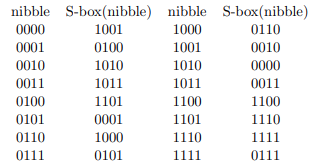
\includegraphics[width = 0.6\linewidth]{Imagens/S-Boxes.png}  
    \label{fig:S-Boxes}
\end{figure}

\subsubsection{ShiftRows}
No nosso modelo simplificado, nessa etapa da encriptação os elementos da segunda linha da matriz de estados são trocados de posição. No \textbf{AES}, o shift das linhas é feito seguindo o número da linha menos 1, isso significa que a primeira linha não é deslocada, a segunda uma única posição a esquerda, a terceira 2 posições, e a quarta 3 posições.

\subsubsection{MixColumns}
Essa é a última função que precisaremos descrever para o processo de encriptação, que é feita por uma multiplicação em \textbf{GF(16)} entre a matriz de estado e a matriz $
\begin{bmatrix}
  1 & 4 \\
  4 & 1
\end{bmatrix}$. Primeiramente, podemos definir a multiplicação	em \textbf{GF(16)} pelo seguinte trecho de código:

\begin{lstlisting}[language=Python]
def gf16_mul(a:int, b:int) -> int:
  result = 0
  for _ in range(4):
    if b & 1:
      result ^= a
    b >>= 1
    a <<= 1
    if a & 0b10000:
      a ^= 0x13
  return result & 0xF
\end{lstlisting}

Já o processo de misturar as colunas da matriz de estado, podemos utilizar o seguinte trecho de código, que basicamente simula a multiplicação de matrizes:

\begin{lstlisting}[language=Python]
def mix_columns(state: list[list[int]]) -> list[list[int]]:
  return [
    [
      gf16_mul(1, state[0][0]) ^ gf16_mul(4, state[1][0]), 
      gf16_mul(1, state[0][1]) ^ gf16_mul(4, state[1][1])
    ],
    [
      gf16_mul(4, state[0][0]) ^ gf16_mul(1, state[1][0]),
      gf16_mul(4, state[0][1]) ^ gf16_mul(1, state[1][1]) 
    ]
  ]
\end{lstlisting}

Já no \textbf{AES}, a matriz utilizada é $$
\begin{bmatrix}
  2 & 3 & 1 & 1 \\
  1 & 2 & 3 & 1 \\
  1 & 1 & 2 & 3 \\
  3 & 1 & 1 & 2
\end{bmatrix}
$$, mantendo o mesmo processo de multiplicação em \textbf{GF(16)} para obter o resultado da operação.

\subsection{Round 1 e 2}
Tendo todas as funções necessárias definidas, além de dos conceitos relacionados com cada um dos mesmos, o processo de encriptação com a S-AES pode ser realizado com sucesso. Desse modo, essa parte do trabalho será dedicada a relembrar e encadear \blue{todo} o processo de encriptação além de apresentar uma sequencia de resultados intermediários que levarão do \textit{plaintext} ao \textit{ciphertext}.

Nesse sentido, podemos definir o fluxo do algoritmo S-AES como sendo o seguinte:
\begin{enumerate}
  \item Realizar a expansão da chave;
  \item Utilizar o Add Round Key com \textit{plaintext} e a chave de entrada;
  \item Inicia a primeira rodada com o SubNibbles do estado obtido anteriormente;
  \item Seguindo com o estado obtido é utilizado o ShiftRows;
  \item Seguindo a mesma sequência, utiliza-se o MixColumns;
  \item Finalizando a primeira rodada, realiza-se o Add Round Key com o estado obtido e a chave da primeira rodada (obtida com a expansão);
  \item Inicia a segunda rodada com o SubNibbles;
  \item Seguido com o ShiftRows;
  \item Diferente da primeira rodada, já finaliza com o Add Round Key com a chave da segunda rodada;
\end{enumerate}

A pequena diferença que ocorre entre a primeira e a segunda rodada, removendo a etapa de mix columns, se deve a intenção de simplificar o processo de decriptação. No \textbf{AES}, além das diferenças já citadas ao longo das análises, não possui essa remoção do mix columns na última rodada. 

Com base nas observações feitas, podemos observar com melhor compreensão os resultados retornados pelo algoritmo resultado da pesquisa até o ponto atual, presenta na imagem \ref{fig:S-AES Results}.

\begin{figure}[h]
    \centering
    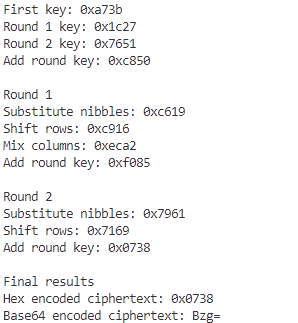
\includegraphics[width = 0.5\linewidth]{Imagens/S-AES-Results.png}  
    \label{fig:S-AES Results}
\end{figure}

\subsection{Modo de operação: ECB}
A técnica utilizada por esse modo de operação é bem simples, consistindo em dividir a entrada fornecida em blocos de tamanho fixo para serem repassados a função de criptografia desejada.

No caso da \textbf{S-AES}, a entrada foi definida como blocos de 16 bits incluindo um padding de \blue{0s} a esquerda no último bloco, em caso de não possuir os 16 bits necessários. No \textbf{AES} o valor dos blocos seria de 128 bits. O código utilizado para essa tarefa foi o seguinte:

\begin{lstlisting}[language=Python]
def encrypt_saes_ecb(text:str, key:int):
  ciphertext = bytearray()
  for i in range(0, len(text), 2):
    block = text[i:i+2]
    if len(block) < 2:
      block = block.ljust(2, '\x00')
    ct = saes(block, key)
    ciphertext += ct.to_bytes(2, byteorder="big")
  return b64.b64encode(ciphertext).decode("utf-8")
\end{lstlisting}

Nele pode ser percebido a divisão em blocos de 2 letras(que totaliza 16 bits) e o padding de 0s a esquerda. Para exemplificar, caso a mensagem passada ao algoritmo seja \textbf{okk} a conversão resultante será o array [0110111101101011, 0000000001101011]. 

Vale lembrar que esse \textbf{não} é o valor retornado pela função, pois nessa função está inclusa a criptografia utilizando o algoritmo \blue{S-AES}. Desse modo, o resultado final será a concatenação de todas os blocos criptografados convertidos no formato da base 64 (melhor legibilidade).

\section{Modos de operação}
Nessa etapa do estudo, será feita a comparação de 5 modos de operação utilizando o algoritmo \textbf{AES}. A biblioteca escolhida para a utilizar as implementações desses modos de operação foi a pyCryptoDome. Nesse primeiro momento, serão detalhados a ideia por trás de cada modo de operação e o resultado obtido em cada uma.

Para melhor comparação, foram utilizadas duas frases a serem encriptadas, para explorar possíveis diferenças no tamanho da frase na aleatoriedade gerada. A primeira foi a mesma utilizada no S-AES, a palavra "ok", e a segunda foi a frase "Uma frase mais comprida para permitir uma melhor comparação entre os diferentes modelos de modo de operação existentes, utilizando o algoritmo AES." que possui 147 caracteres de comprimento (ou 1176 bits).

\subsection{ECB - Electronic CodeBook}
Como foi definido anteriormente nesse trabalho, essa função consiste em receber um texto de entrada e converte-lo em blocos de texto de tamanho fixo (no caso do S-AES 16 bits) para serem criptografados e concatenados em uma única mensagem final.

\begin{figure}[h]
    \caption{ECB com frase curta}
    \centering
    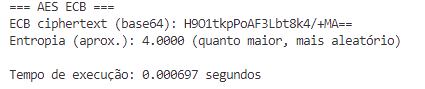
\includegraphics[width = 0.5\linewidth]{Imagens/ECB-curto.png}  
    \label{fig:ECB Curto}
\end{figure}

\begin{figure}[h]
    \caption{ECB com frase longa}
    \centering
    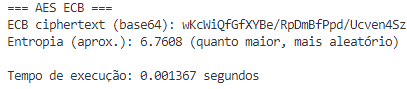
\includegraphics[width = 0.5\linewidth]{Imagens/ECB-longo.png}  
    \label{fig:ECB Longo}
\end{figure}

Com base no que pode ser visto nas imagens \ref{fig:ECB Curto} e \ref{fig:ECB Longo}, podemos observar que o grau de aleatoriedade teve um aumento de pouco mais de 50\% da frase curta para a frase longa e o tempo de processamento foi dobrado. Visto que esse modo de operação \blue{possui padding}, o tamanho da frase curta foi de 128 bits e a frase longa 1280 bits, logo é 10 vezes maior e dessa forma os aumentos relatados são bem menores do que o aumento da própria frase.

\subsection{CBC - Cipher-block chaining}
Nesse modo de operação, além da mensagem dividida em blocos de X bits (fixos) e da chave de X bits também será recebida um valor inicial (IV), que será utilizado para realizar o XOR com o primeiro bloco da mensagem a ser encriptada. Esse modo de operação utiliza o bloco cifrado anterior para realizar um XOR com a entrada seguinte.

Um problema presente nesse modo de operação é a propagação de erros caso algum bit seja alterado na transmissão, afetando toda a cadeia de decriptação da mensagem.

\begin{figure}[h]
    \caption{CBC com frase curta}
    \centering
    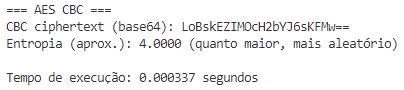
\includegraphics[width = 0.5\linewidth]{Imagens/CBC-curto.png}  
    \label{fig:CBC Curto}
\end{figure}

\begin{figure}[h]
    \caption{CBC com frase longa}
    \centering
    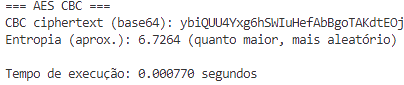
\includegraphics[width = 0.5\linewidth]{Imagens/CBC-longo.png}  
    \label{fig:CBC Longo}
\end{figure}

Com base no que pode ser visto nas imagens \ref{fig:CBC Curto} e \ref{fig:CBC Longo}, podemos observar que o grau de aleatoriedade e o tempo de processamento teve aumento similar ao observado no ECB.

\subsection{CFB - Cipher feedback}
Nesse modo de operação, a entrada é cifrada de forma similar a feita no \blue{CBC}, realizando XOR da entrada a ser encriptada com outro valor. A principal diferença está em cifrar o valor inicial ou o bloco anterior usando o \textbf{AES} antes de realizar o XOR com o próximo bloco em texto puro. A cifragem pode ser descrita com o seguinte exemplo, sendo C o texto cifrado e P o \textit{plaintext}:
\begin{itemize}
  \item C$_{1}$ = AES(IV) XOR P$_{1}$
  \item C$_{2}$ = AES(C$_{1}$) XOR P$_{2}$
  \item C$_{3}$ = AES(C$_{2}$) XOR P$_{3}$
  \item \dots
\end{itemize}

Outra característica interessante é ser capaz de aceitar blocos de entrada de tamanhos variados, não se fazendo necessário o uso de padding. No entanto, possui o mesmo problema de 

\begin{figure}[h]
    \caption{CFB com frase curta}
    \centering
    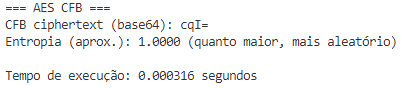
\includegraphics[width = 0.5\linewidth]{Imagens/CFB-curto.png}  
    \label{fig:CFB Curto}
\end{figure}

\begin{figure}[h]
    \caption{CFB com frase longa}
    \centering
    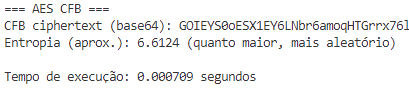
\includegraphics[width = 0.5\linewidth]{Imagens/CFB-longo.png}  
    \label{fig:CFB Longo}
\end{figure}

Com base no que pode ser visto nas imagens \ref{fig:CFB Curto} e \ref{fig:CFB Longo}, podemos observar que o tempo de processamento teve aumento similar ao observado nos outros modos, mas a aleatoriedade do texto foi muito menor no texto curto, isso se deve a ausência de padding, que manteve o texto bem curto, sem a possibilidade de grandes diferenças por parte do modo de operação no efeito criptográfico.

\subsection{OFB - Output feedback}
Agora no OFB vamos observar outro modo com bastante semelhança com o \textbf{CBC} e o \textbf{CFB}. A diferença nesse modelo está em qual a parte que fara o XOR com o \textit{plaintext}, utilizando também uma parte que já foi cifrada desde o inicio, diferenciando do \blue{CBC}, mas que não é o bloco anterior sendo essa a diferença do \blue{CFB}. A cifragem pode ser descrita com o seguinte exemplo, sendo C o texto cifrado, P o \textit{plaintext} e O um valor auxiliar:
\begin{itemize}
  \item O$_{1}$ = AES(IV)
  \item C$_{1}$ = O$_{1}$ XOR P$_{2}$ => Igual ao CFB até aqui
  \item O$_{2}$ = AES(O$_{1}$)
  \item C$_{3}$ = O$_{2}$ XOR P$_{3}$
  \item \dots
\end{itemize}

Nesse modo de operação temos algumas vantagens, como a possibilidade de paralelizar a cifragem de um bloco com o de outros, visto que um não tem mais dependência direta com o outro, o que também retira o problema do modo anterior de propagação de erros na decriptação, em caso de falha na transmissão da mensagem. No entanto, o valor de O ainda depende do anterior, o que limita a possibilidade de paralelização. 

\begin{figure}[h]
    \caption{OFB com frase curta}
    \centering
    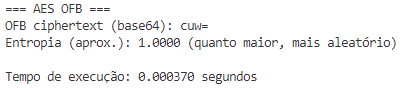
\includegraphics[width = 0.5\linewidth]{Imagens/OFB-curto.png}  
    \label{fig:OFB Curto}
\end{figure}

\begin{figure}[h]
    \caption{OFB com frase longa}
    \centering
    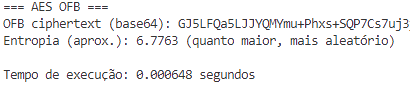
\includegraphics[width = 0.5\linewidth]{Imagens/OFB-longo.png}  
    \label{fig:OFB Longo}
\end{figure}

Com base no que pode ser visto nas imagens \ref{fig:OFB Curto} e \ref{fig:OFB Longo}, os valores seguem o que ocorreu no \blue{CFB}, porém com o aumento no tempo discretamente menor.

\subsection{CTR - Counter}
Esse modo consegue superar o problema de paralelização do \textbf{OFB}, mantendo as vantagens já apontadas. Esse processo se faz possível por meio de um contador que é acrescido a chave de inicialização utilizada, que pode ter seu valor determinado para todos os blocos a serem cifrados antes mesmo de iniciar a primeira encriptação dessa soma. Para contextualizar podemos ver a seguinte sequência:

\begin{itemize}
  \item K$_{1}$ = AES(IV + 0)
  \item C$_{1}$ = K$_{1}$ XOR P$_{2}$ => Igual ao CFB/OFB até aqui
  \item K$_{2}$ = AES(IV + 1)
  \item C$_{3}$ = K$_{2}$ XOR P$_{3}$
  \item \dots
\end{itemize}

\begin{figure}[h]
    \caption{CTR com frase curta}
    \centering
    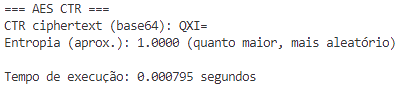
\includegraphics[width = 0.5\linewidth]{Imagens/CTR-curto.png}  
    \label{fig:CTR Curto}
\end{figure}

\begin{figure}[h]
    \caption{CTR com frase longa}
    \centering
    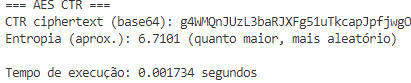
\includegraphics[width = 0.5\linewidth]{Imagens/CTR-longo.png}  
    \label{fig:CTR Longo}
\end{figure}

Com base no que pode ser visto nas imagens \ref{fig:CTR Curto} e \ref{fig:CTR Longo}, os valores seguem o que ocorreu no \blue{CFB}, porém vale levantar que o tempo necessário foi bem maior do que em outros modos.

\subsection{Observações}
Comparando todos os modos, pode ser observado que o modo "mais rápido" seria o ECB, dada a sua simplicidade, sem chaves extras, nem criptografias/XORs extras. Por outro lado, esse modo não incrementa o grau de segurança da criptografia utilizada. 

Levando isso em conta, o modelo que possivelmente que se destaca é o CTR, baseado na sua possibilidade de paralelização, o que permite ganho na velocidade, mantendo um grau de segurança similar os dos outros 3 modos restantes. Porem, foi observado quem em textos curtos (menos que milhares de caracteres) essa sua vantagem de paralelização não foi muito significativa e ainda levou a uma perda de performance em comparação com os demais modos.

Por fim, o grau de aleatoriedade, segundo o método que foi estabelecida no código, que pode ser encontrado na seção \ref{codigos}, se encontrou muito similar entre todos os métodos ao utilizar textos maiores, onde o padding não fez grande diferença. 

Desse modo, o ganho na segurança da mensagem não é perceptível ao utilizar métodos que olham unicamente por frequência de termos, visto que o próprio \blue{AES} lida bem com esse problema, camuflando bem a diferença entre os modos nos restando principalmente a análise da teoria por trás de cada método para ver suas diferenças. 

\section{Código}
O código está disponível no github pelo link: \href{https://github.com/Diehlgit/S-AES}{https://github.com/Diehlgit/S-AES}

\end{document}